\section{Generalizing to Categorical-Valued $\theta$}
For the experiment described in this chapter, 
we relax the assumption made in Chapter \ref{chapter:cocktail-party} 
that the $\theta_j$ are binary vectors and
instead allow each $\theta_{jd}$ to take on one in an arbitrary set of
discrete values --- i.e., to be categorically distributed rather than
Bernoulli distributed; however the similarity between two states will again be defined in terms of distance between $\theta_j$ vectors that also inform the emission distribution via a linear-Gaussian model.  As a result, much of the additional inference steps described for the 
cocktail party experiment carry over here.  The exception of course is
inferences about $\theta$.

In this chapter, I first define representations and priors for $\theta$ and the weight matrix, 
$W$ for the general case of categorical-vector-valued $\theta$.  Then I derive the necessary Gibbs steps.  Finally, I describe an application to power disaggregation, where the observations consists of an aggregated energy-use time series from several houses, the latent state vector describes the energy being used by each of several channels (e.g., lighting, refrigerator, washer/dryer), such that individual channels are in one of several discrete states at a given time. For example, the refrigerator channel might cycle between an ``off'' state, a low-power standby state, and a high-power ``active cooling'' state.  Inference consists of discovering the set of discrete states for each channel, attributing a typical level of energy consumption for each state, and inferring what state each channel is in during each discretized time window in the data.

\section{Priors and Representations in the Categorical State Variant}
\label{sec:priors-repr-categ}

In place of Beta priors on each $\theta_{jd}$, we use Chinese
Restaurant Process priors, with concentration parameter
$\alpha_{d}^{(\theta)}$.  In the case that the number of categorical 
values is known in advance, this can be replaced by a Dirichlet 
prior, but I present the more flexible case here. 

The weight matrix $W$ must be expanded to allow for distinct weights
associated with each possible value of the $\theta_{jd}$.  Rather than
the matrix given by $(w_{dk})_{d=1,\dots,D,k=1,\dots,K}$, we now need
a set of weights, $(w_{sdk})$, where $s$ indexes the categorical
values that $\theta_{jd}$ can take.  With a CRP prior, 
there is an unbounded number of $s$, though during inference, as in the direct assignment sampler for the HDP-HMM, we need only consider those values to which some state is currently assigned, plus one additional value representing a ``new'' state.

I will continue to assume that the $\phi$ function
decays exponentially as a function of the number of component-wise
differences (that is, Hamming distance) 
between a pair of states.  Specifically, $\Delta_{jj'd}$ is zero
if and only if $\theta_{jd} = \theta_{j'd}$ and is 1 otherwise,
$\Delta_{jj'} = \sum_{d} \Delta_{jj'd}$, and
$\phi(\theta_{j}\theta_{jj'}) = e^{-\lambda\Delta_{jj'}}$.
  
We can use a ``dummy variable'' representation
of $\theta_j$.  Define $S_d$ to be the number of realized
states for dimension $d$ and a 1 in position $\sum_{d' < d} S_{d'} + s$ indicates that
$\theta_{jd} = s$.  There will thus be $D$ entries equal to 1, with
the remaining entries equal to zero.  We can then represent the weight
matrix $\bW$ as stacked block matrix, where each block is $S_d
\times K$, and there is one block for each $d$.  In practice we only
need to instantiate a new block when some $\theta_{jd}$ is assigned to
a ``new table'' in the CRP metaphor, so that the dimension of $\bW$ is
$\sum_d S_d \times K$.  Then we have
\begin{equation}
  y_{t} \sim \Norm{w^{(b)} + W^{\sf T}\theta_{z_t}}{\Sigma}
\end{equation}
where $w^{(b)}$ is a $K$-dimensional bias vector with a separate Normal
prior, $W$ is the weight matrix as defined just above, $z_t$ is the
state indicator for time $t$, and $\Sigma$ is a $K \times K$ noise covariance matrix.

\section{Adapting Posterior Inference for Categorical State Vectors}
\label{sec:adapt-post-infer}

\subsubsection{Sampling $\theta$}

As before, the conditional posterior for $\theta_{jd}$ 
is proportional to the product of three terms: the prior (now a CRP),
the likelihood of all successful and failed transitions to and from
state $j$, and the likelihood of the observation sequence.

Under the CRP, the probability that $\theta_{jd} = s$ conditioned on the rest of $\theta$ (but not the data) is proportional to the number of other $j' \neq j$ such that
$\theta_{j'd} = s$ where this count is positive; and proportional to
$\alpha_j^{(\theta)}$ otherwise.  Let 
\begin{equation}
\tilde{n}^{-j}_{ds} = \sum_{j' \neq j} I(\theta_{jd} = s), \quad s = 1,
\dots, S_d
\end{equation}
be these counts, where we assume that there are $S_d$ distinct values
taken by the $\theta_{jd}$ for a particular $d$.  Then
\begin{equation}
  p(\theta_{jd} = s \given \theta_{d}^{-j}) \propto
\begin{cases}
\tilde{n}^{-j}_{ds} & s = 1, \dots, S_d \\
\alpha_{d}^{(\theta)} & s = S_d + 1
\end{cases}
\end{equation}

The transition component of the likelihood is as in the binary case:
\begin{align}
  p(z, Q \given \theta_{jd}, \theta_{d}^{-j}) & \propto
  e^{-\lambda\sum_{j'} \Delta_{jj'} (n_{jj'} + n_{j'j})} \prod_{j'
    \neq j} (1 - e^{-\lambda\Delta_{jj'} (q_{jj'} + q_{j'j})})\\
  &\propto e^{-\lambda \sum_{j'} I(\theta_{jd} \neq \theta_{j'd})
    (n_{jj'} + n_{j'j})} \prod_{j'
    \neq j} (1 - a\cdot e^{-\lambda I(\theta_{jd} \neq \theta_{j'd}) (q_{jj'} + q_{j'j})})
\end{align}
where $a$ is a constant in $\theta_{jd}$, defined as $e^{-\lambda
  \Delta_{jj'-d} (q_{jj'd} + q_{j'jd})}$.  Taking a log yields
\begin{equation}
  \log p(z, Q \given \theta_{jd}, \theta_{d}^{-j}) =
  -\lambda \sum_{\{j':\ \theta_{jd} \neq \theta_{j'd}\}} (n_{jj'} +
  n_{j'j}) + \sum_{j'
    \neq j} \log(1 - a\cdot e^{-\lambda I(\theta_{jd} \neq \theta_{j'd}) (q_{jj'} + q_{j'j})})
\end{equation}

The emission component of the likelihood is given for each $t$ by
\begin{equation}
  p(y_t \given \theta_{z_t}, W, \Sigma) \propto \abs{\Sigma}^{-1/2}
  \exp(-\frac{1}{2} (y_t - w^{(b)} -
  W^{\sf T} \theta_{z_t})^{\sf T}\bSigma^{-1}(y_t - w^{(b)} - W^{\sf T} \theta_{z_t}))
\end{equation}

Assuming a diagonal covariance matrix, isolating $\theta_{j,d}$, and
taking a log, this becomes, for each $k$ and $t$,
\begin{align}
  \log p(y_{tk} \given \theta_{z_t,d}, \theta_{z_t}^{-d}, w^{(b)}_k, \sigma^2_k) &=
   -\frac{1}{2\sigma^2_k} \left(y_{tk} -
      w^{(b)}_k-\theta_{z_t}\bw_k\right)^2 \\
  &\propto -\frac{1}{2\sigma^2_k} (\sum_{d'} w_{\theta_{z_td'},d',k} -
    (y_{tk} - w^{(b)}_k))^2 \\
  &\propto -\frac{1}{2\sigma^2_k}(w_{\theta_{z_td},d,k} - (y_{tk} -
    w^{(b)}_k - \sum_{d' \neq d} w_{\theta_{z_t,d'},d',k}))^2
\end{align}
For a particular $j$ and $d$, the full emission log likelihood is a sum of
terms like the above, over all $t$ such that $z_t = j$.

\paragraph{Sampling $W$}
Having expanded $\theta$ to a dummy variable representation, and
having constructed a stacked block form of $W$, we can sample each
column of $W$ from a conditional posterior multivariate Normal just
as in the binary case.

\paragraph{Sampling $\lambda$} Since $\lambda$ controls only the relationship between the distance matrix, $\Delta$, and the similarity matrix, $\phi$, upon 
conditioning on $\Delta$ and the jump attempts, $\lambda$ is not sensitive to the way that $\Delta$ was computed; hence it can be sampled using Adaptive Rejection Sampling from exactly the same conditional distribution as before.

\section{Power Disaggregation}
\label{sec:power-disaggregation}

The categorical model was tested using a subset of the Reference Energy Disaggregation Data set (REDD; \citet{kolter2011redd}).  The data consists of power consumption measurements from several time intervals from several electrical channels in several different homes, as well as an aggregated power consumption time series for each interval per home. An example interval is shown in Fig. \ref{fig:redd-data-example}.  

Two key properties of this data are apparent in the figure.  First, up to some small-scale variability, each channel visits a relatively small number of amplitudes, with some (such as the oven) alternating between an ``on'' state and an ``off'' state, and others (such as the outlets and lighting channels) exhibiting more complex dynamics, presumably corresponding to various appliances or light fixtures turning on and off in different combinations.  This property motivates the choice of a categorical state model.  Second, there are clear correlations among the various channels: in this example, the two oven channels always go on and off together, albeit exhibiting different amplitudes when on, while two of the three lighting channels are highly but not perfectly correlated, while the third exhibits opposing behavior to the other two (perhaps arising from behavior).

Collectively, the dynamics exhibited here are similar to the cocktail party data described in Chapter \ref{chapter:cocktail-party}.  For one, since transitions between combinatorial states tend to be ``local'', in that it is rare for more than one channel to change state at one time, we would expect the HaMMLeT model's bias toward local state transitions to be beneficial, compared to the ``vanilla'' HDP-HMM which has no such locality bias.  On the other hand, not all combinations of states occur in the data, and morever, some state combinations are more or likely than the product of the individual channel probabilities would suggest, suggesting that the flexibility of a model such as HaMMLeT, in which there is a single latent state space over vector-valued states, might be better able to capture the correct transition probaiblities than a model such as the Factorial HMM, in which the component chains evolve {\em a priori} independently.

\begin{figure}[tb]
  \centering
  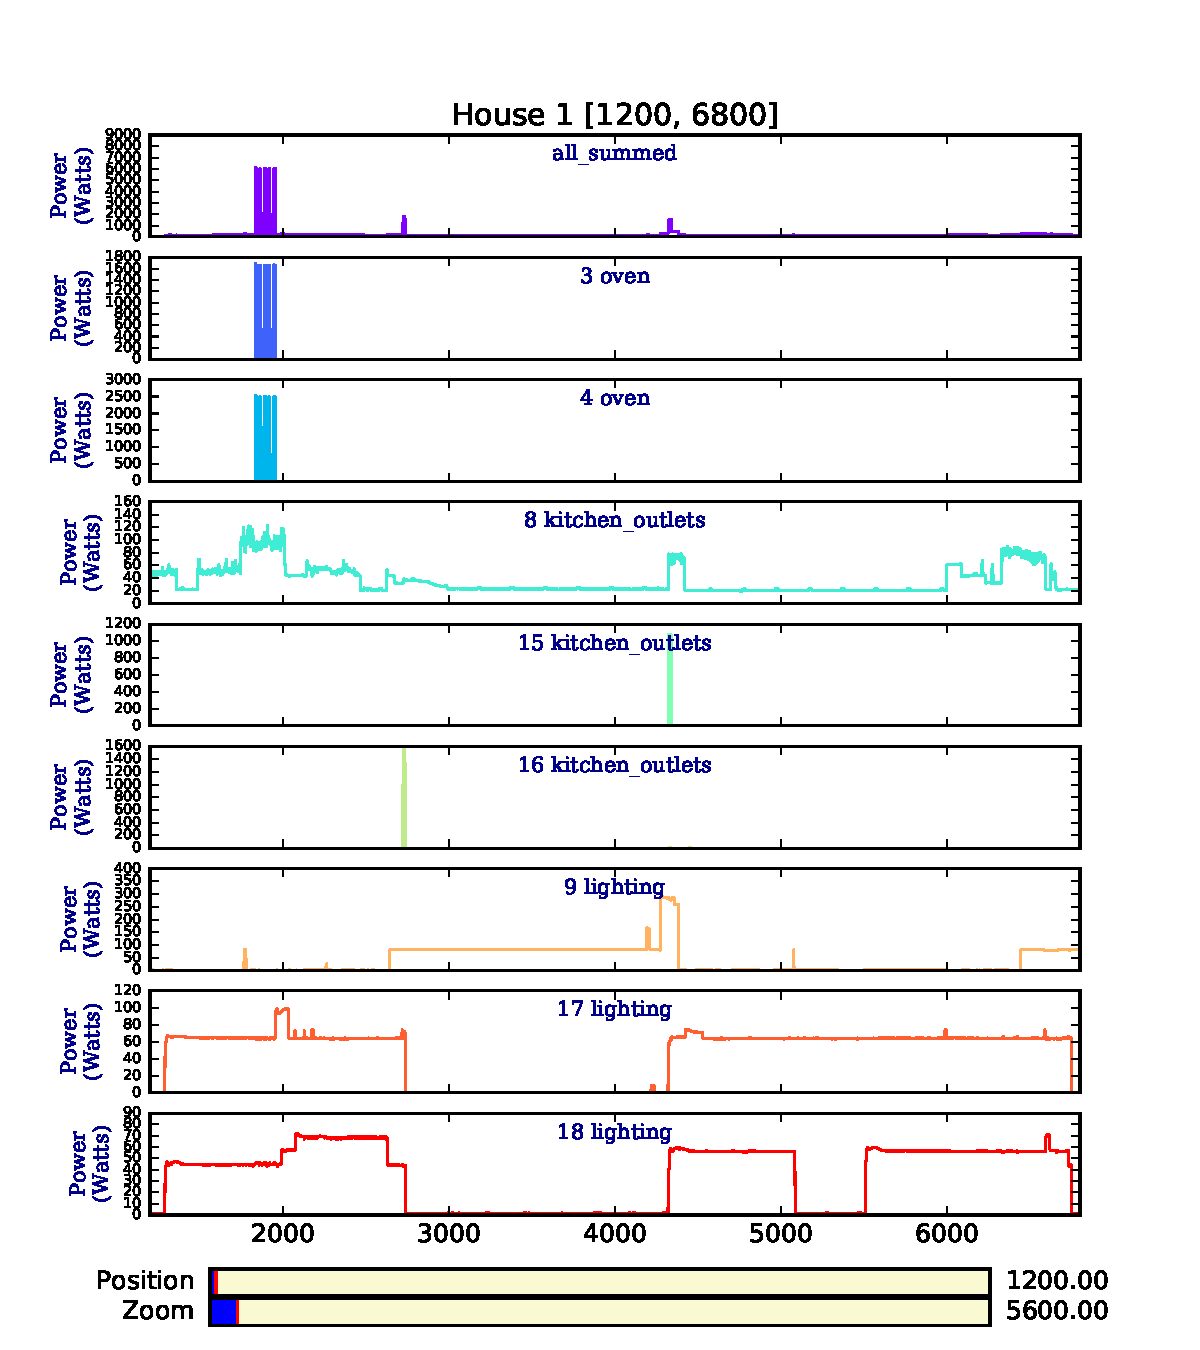
\includegraphics[width=\textwidth]{data/REDD/jw2013_downsampled_intervals/house_1_1200_6800/house_1_1200-6800.pdf}
  \caption{A sample data interval from the REDD dataset \cite{kolter2011redd}.  The top channel contains the total measured power in watts consumed by a home during a period of approximately 24 hours.  Each timestep represents a 20 second intervals, during which the amplitude recorded is a median of the amplitudes in the original higher resolution data.}
  \label{fig:redd-data-example}
\end{figure}